\documentclass[12pt]{article}
\usepackage{geometry}                % See geometry.pdf to learn the layout options. There are lots.
\geometry{letterpaper}                   % ... or a4paper or a5paper or ... 
%\geometry{landscape}                % Activate for for rotated page geometry
\usepackage[parfill]{parskip}    % Activate to begin paragraphs with an empty line rather than an indent
\usepackage{daves,fancyhdr,natbib,graphicx,dcolumn,amsmath,lastpage,url}
\usepackage{amsmath,amssymb,epstopdf,longtable}
\usepackage[final]{pdfpages}
\DeclareGraphicsRule{.tif}{png}{.png}{`convert #1 `dirname #1`/`basename #1 .tif`.png}
\pagestyle{fancy}
\lhead{CE 5364 -- Groundwater Transport Phenomena }
\rhead{FALL 2024}
\lfoot{ES4}
\cfoot{}
\rfoot{Page \thepage\ of \pageref{LastPage}}
\renewcommand\headrulewidth{0pt}



\begin{document}
\begin{center}
{\textbf{{ CE 5364 Groundwater Transport Phenomena } \\ {Exercise Set 4}}}
\end{center}

\section*{\small{Exercises}}
\begin{enumerate} %% Problem Counter

%%%%%%%%%%%%%%%%%%%%%%%%%%%%%%%%%%%%%%%%%%%%%%%%%%%%

\item 

A fuel mixture of benzene, toluene, ethylbenzene at mole fractions 0.075, 0.065, and 0.035 respectively equilibrates with the atmosphere at 25$^oC$

\begin{figure}[h!] %  figure placement: here, top, bottom, or page
   \centering
   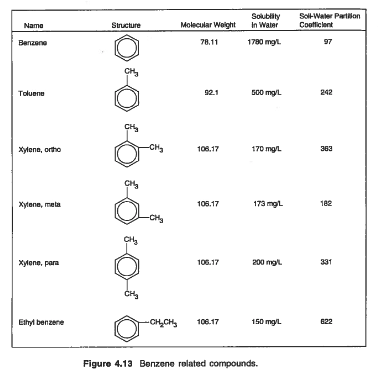
\includegraphics[width=5in]{Fig4-13.png} 
   \caption{Benzene Compounds - Structural diagrams and physical properties}
   \label{fig:plumemap}
\end{figure}

\begin{figure}[h!] %  figure placement: here, top, bottom, or page
   \centering
   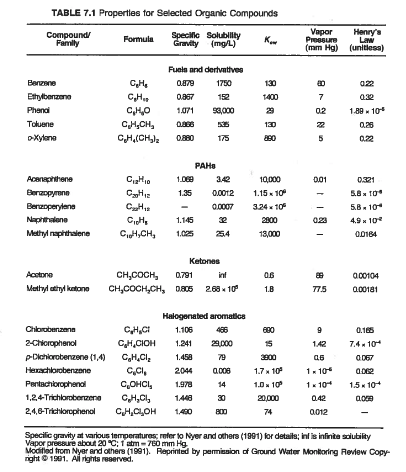
\includegraphics[width=5in]{Tab7-1.png} 
   \caption{Physical properties for some organic compounds}
   \label{fig:plumemap}
\end{figure}

\newpage
Determine:
\begin{enumerate} %% Deliverable Counter
\item Concentration in the gas (air) phase of the three components in $\frac{mg}{L}$
\item Concentration in the gas (air) phase of the three components in $\frac{\mu g}{m^3}$
%\item The volumetric flow rate through the column.
\end{enumerate} %% Deliverable Counter
\clearpage

%%%%%%%%%%%%%%%%%%%%%%%%%%%%%%%%%%%%%%%%%%%%%%%%%%%%%%%%%%
\item (Modified from 6.22 pg. 592)

A well with effective diameter of 0.5 m fully penetrates an aquifer that has a uniform saturated thickness of 10 m.  One hundred grams of benzene are spilled into the well, immediately dissolve, and mix into the water in the well. The seepage velocity is 30 m/yr in the x-direction, the longitudinal dispersivity is 1.0 m, and the transverse dispersivity is 0.1 m.

The aquifer has the following characteristics: 

\begin{itemize} %% Deliverable Counter
\item Bulk density = 1.8 g/cc
\item porosity = 0.30
\item $f_{oc}$ =  1 percent
\item $K_{ow}$ = 135 L/kg
\end{itemize} %% Deliverable Counter

Determine:
\begin{enumerate} %% Deliverable Counter
\item The retardation factor R for benzene in this aquifer.  
\item The maximum benzene concentration at t = 1 yr.
\item The location of this maximum.
\end{enumerate} %% Deliverable Counter
\clearpage
%%%%%%%%%%%%%%%%%%%%%%%%%%%%%%%%%%%%%%%%%%%%%%%%%%%%%%
%%%%%%%%%%%%%%%%%%%%%%%%%%%%%%%%%%%%%%%%%%%%%%%%%%%%%%
\item 

The following data for concentration of TCE were taken at a single monitoring well.  Use the Mann-Kendall test (pp. 458-460) to determine whether the concentration has an upward or downward trend.

\begin{table}[htbp]
\centering
\caption{TCE Observations in an Aquifer}
\begin{tabular}{p{1.5in}p{1.5in}} % Column formatting, @{} suppresses leading/trailing space
~&~\\
Date&TCE (ppb)\\
\hline
\hline
9/92&8\\
12/92&19\\
3/93&21\\
6/93&13\\
9/93&39\\
12/93&24\\
3/94&28\\
6/94&25\\
\hline
\end{tabular}
\label{tab:TCEobserve}
\end{table}

Determine:
\begin{enumerate} %% Deliverable Counter
\item The upward or downward concentration trend, using a Mann-Kendall test.
\end{enumerate} %% Deliverable Counter

%%%%%%%%%%%%%%%%%%%%%%%%%%%%%%%%%%%%%%%%%%%%%%%%%%%%%%%%%%%%%%%%%%%
\end{enumerate}%% Problem Counter

\end{document}  